\chapter{Assignment: Overfitting}
\label{hw:overfitting}

\newthought{Overfitting is something we try to avoid at all times.} But overfitting comes in many shapes and sizes. For this exercise we will use a \emph{blood-loneliness} data set with the File widget. This data set relates gene expressions in blood with a measure of loneliness obtained from a sample of elderly persons. Let's try to model loneliness with logistic regression and see how well the model performs.

\marginnote{To load the blood loneliness data set copy and paste the below URL to the URL field of the File widget.
\break\break
\url{http://file.biolab.si/datasets/blood-loneliness-GDS3898.tab}}

\begin{figure}[h]
  \centering
  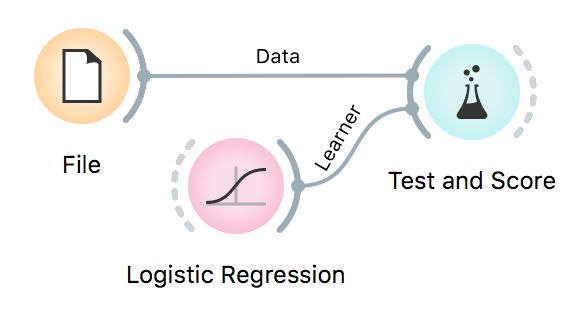
\includegraphics[scale=0.7]{overfitting1.png}%
  \caption{$\;$}
  \label{fig:wf1}
\end{figure}

\begin{enumerate}
    \item Train the Logistic Regression model on the data and observe its performance. What is the result?
    \item We have many features in our data. What if we select only the most relevant ones, the genes that actually matter? Use Rank to select the top 20 best performing features.
    
    \begin{figure}[h]
        \centering
        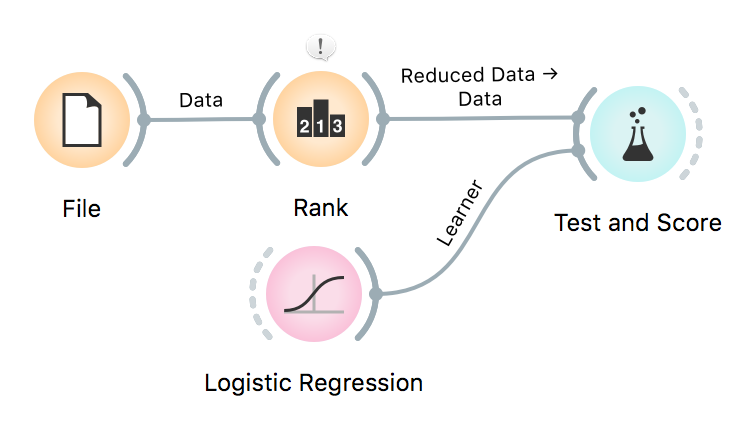
\includegraphics[scale=0.7]{overfitting2.png}%
        \caption{$\;$}
        \label{fig:wf2}
      \end{figure}

    \item How are the results now? What happened? Is there a better way of performing feature selection?
\end{enumerate}
